\documentclass{fkssolpub}

\usepackage[czech]{babel}
\usepackage{fontspec}
\usepackage{fkssugar}
\usepackage{amsmath}
\usepackage{graphicx}

\author{Ondřej Sedláček}
\school{Gymnázium Oty Pavla} 
\series{74-I}
\problem{4} 

\begin{document}

\begin{figure}
	\begin{center}
		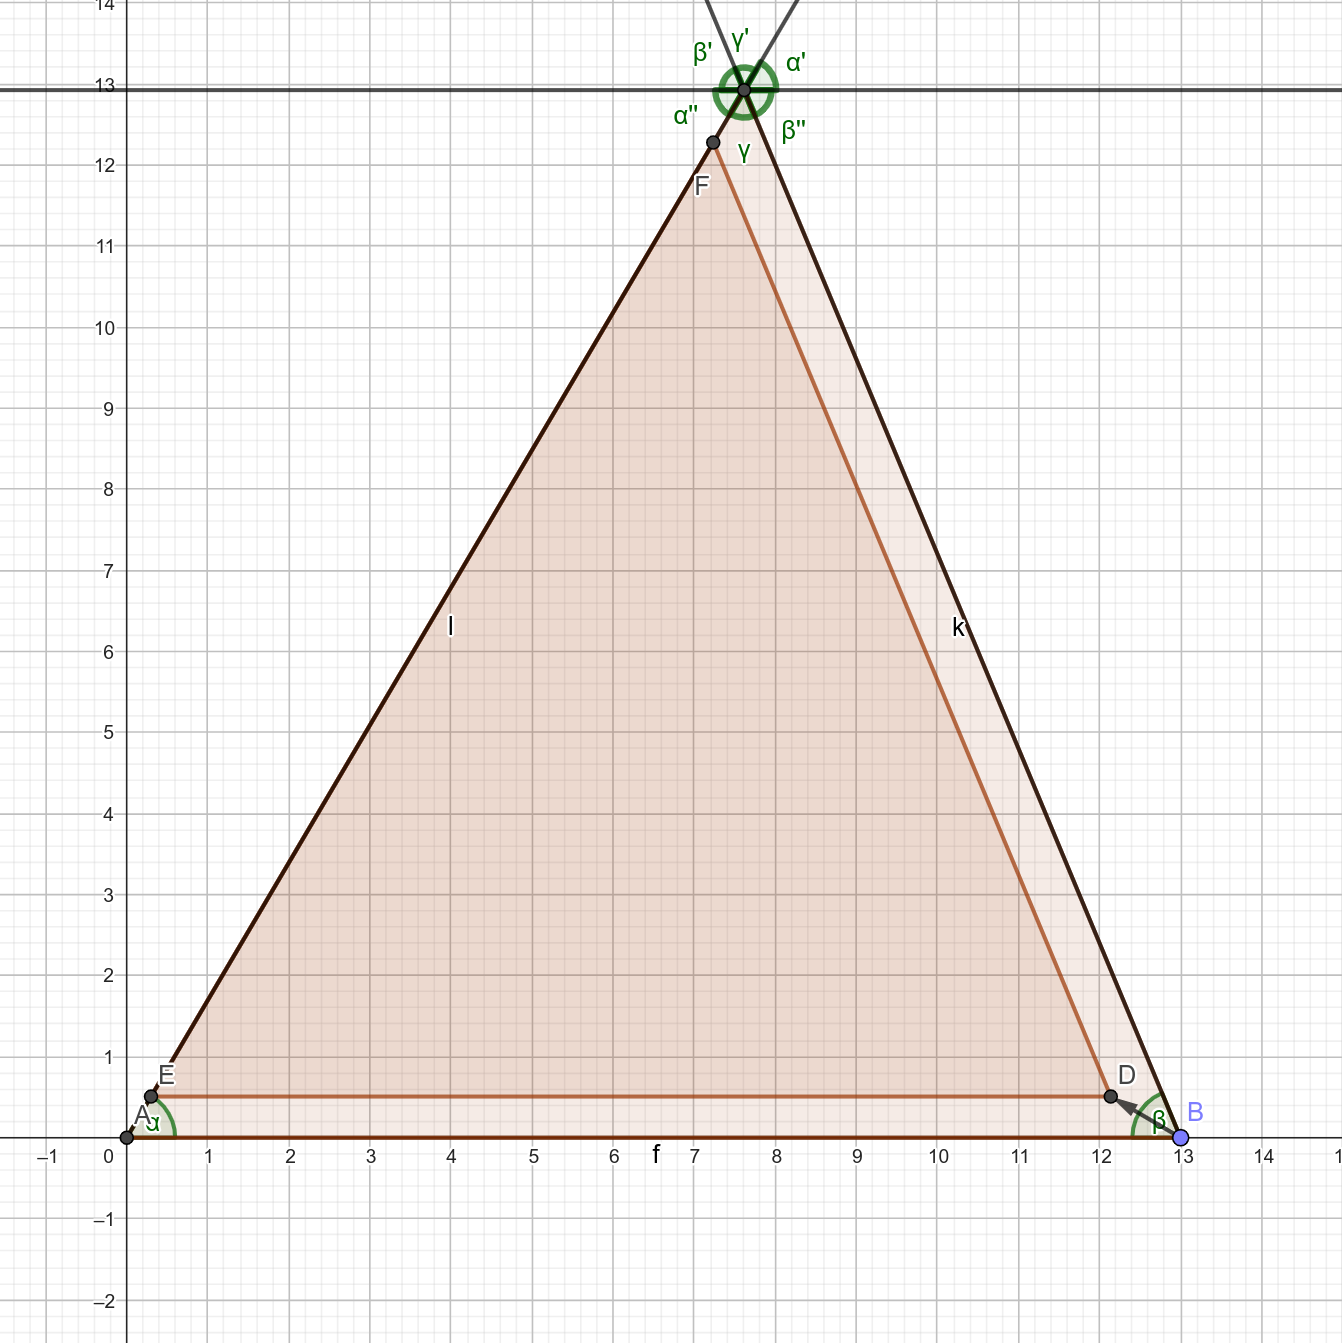
\includegraphics[width=0.75\textwidth]{4-fig}
	\end{center}
	\caption{Konstrukce, při kterým je obsah průniku nejmenší}
	\label{fig:1}
\end{figure}


Jako první si musíme uvědomit, že průnik trojúhelníků $ABC$ a $A'B'C'$ je nutně těmto trojúhelníkům podobný. To můžeme ukázat pomocí věty uu -- každá strana průniku je rovnoběžná s příslušnými stranami trojúhelníků $ABC$ a $A'B'C'$, tím pádem se jejich úhly musí shodovat.

Teď budeme uvažovat případ, kdy když počátek vektoru dosadíme do jednoho z vrcholů $A$, $B$, $C$ (dál budu bez újmy na obecnost uvažovat vrchol $A$), tak bude vektor mířit dovnitř trojúhelníku $ABC$. Pak jeden z vrcholů průniku bude $A'$ a protější strana $x$ bude ležet na úsečce $BC$. Proto bude obsah roven $S = \frac{1}{2} \cdot |x| \cdot |A'; x|$. Z podobnosti zároveň víme, že každá strana a výška průniku trojúhelníků se zmenší $k$-krát, proto když zminimalizujeme $|A'; x|$, tak zminimalizujeme i $|x|$. To nastane právě tehdy, když celý vektor bude ležet na výšce průniku z bodu $A'$. Proto v tomto případě je tedy nejmenší obsah průniku tehdy, kdy vektor leží na nejkratší výšce, když jeho počátek dáme do jednoho z vrcholů původního trojúhelníku.

Toto zjištění ale bude platit taky i v ostatních případech. Stačí nám jenom pozorování, že průnik u vektorů opačného směru je stejný, protože u opačných vektorů nám stačí prohodit $A$ za $A'$, $B$ za $B'$ a $C$ za $C'$ a dostaneme zase vektor, který míří do trojúhelníku. Tyto dva případy pokrývají veškeré případy, protože když přeneseme úhly, kde vektory v obou těchto případech leží, pokryjeme celých $360 ^{\circ}$. Pro nalezení nejmenšího průniku tedy musíme najít nejkratší výšku a tu zkrátit.

Obsah trojúhelníku $ABC$ spočítáme jako:
\[
	S_{ABC} = \frac{1}{4} \sqrt{(13 + 14 + 15) (13 + 14 - 15) (13 - 14 + 15) (-13 + 14 + 15)} = 84
\]
Nejkratší výška je pak výška vůči nejdelší straně, proto nejkratší výška je $v_{CA} = \frac{2 S_{ABC}}{|CA|} = \frac{56}{5}$. Koeficient, o který se pak změní délka všech stran, bude $k = \frac{v_{CA} - 1}{v_{CA}} = \frac{51}{56}$. Pak obsah průniku bude $S = k^2 S_{ABC} = \frac{7803}{112} \doteq 69{,}67$. Tento obsah je tedy nejmenší, který můžeme najít.

\end{document}
